\documentclass{article}
\usepackage{fullpage}
\usepackage[utf8]{inputenc}
\usepackage{pict2e}
\usepackage{amsmath}
\usepackage{enumitem}
\usepackage{eurosym}
\usepackage{mathtools}
\usepackage{amssymb, amsfonts, latexsym, cancel}
\setlength{\parskip}{0.3cm}
\usepackage{graphicx}
\usepackage{fontenc}
\usepackage{slashbox}
\usepackage{setspace}
\usepackage{gensymb}
\usepackage{accents}
\usepackage{adjustbox}
\setstretch{1.35}
\usepackage{bold-extra}
\usepackage[document]{ragged2e}
\usepackage{subcaption}
\usepackage{tcolorbox}
\usepackage{xcolor, colortbl}
\usepackage{wrapfig}
\usepackage{empheq}
\usepackage{array}
\usepackage{parskip}
\usepackage{arydshln}
\graphicspath{ {images/} }
\renewcommand*\contentsname{\color{black}Índice} 
\usepackage{array, multirow, multicol}
\definecolor{lightblue}{HTML}{007AFF}
\usepackage{color}
\usepackage{etoolbox}
\usepackage{listings}
\usepackage{mdframed}
\setlength{\parindent}{0pt}
\usepackage{underscore}
\usepackage{hyperref}
\usepackage{tikz}
\usepackage{tikz-cd}
\usetikzlibrary{shapes, positioning, patterns}
\usepackage{tikz-qtree}
\usepackage{biblatex}
\usepackage{pdfpages}
\usepackage{pgfplots}
\usepackage{pgfkeys}
\addbibresource{biblatex-examples.bib}
\usepackage[a4paper, left=1cm, right=1cm, top=1cm,
bottom=1.5cm]{geometry}
\usepackage{titlesec}
\usepackage{titletoc}
\usepackage{tikz-3dplot}
\usepackage{kbordermatrix}
\usetikzlibrary{decorations.pathreplacing}
\newcommand{\Ej}{\textcolor{lightblue}{\underline{Ejemplo}}}
\setlength{\fboxrule}{1.5pt}

% Configura el formato de las secciones utilizando titlesec
\titleformat{\section}
{\color{red}\normalfont\LARGE\bfseries}
{Tema \thesection:}
{10 pt}
{}

% Ajusta el formato de las entradas de la tabla de contenidos
\addtocontents{toc}{\protect\setcounter{tocdepth}{4}}
\addtocontents{toc}{\color{black}}

\titleformat{\subsection}
{\normalfont\Large\bfseries\color{red}}{\thesubsection)}{1em}{\color{lightblue}}

\titleformat{\subsubsection}
{\normalfont\large\bfseries\color{red}}{\thesubsubsection)}{1em}{\color{lightblue}}

\newcommand{\bboxed}[1]{\fcolorbox{lightblue}{lightblue!10}{$#1$}}
\newcommand{\rboxed}[1]{\fcolorbox{red}{red!10}{$#1$}}

\DeclareMathOperator{\N}{\mathbb{N}}
\DeclareMathOperator{\Z}{\mathbb{Z}}
\DeclareMathOperator{\R}{\mathbb{R}}
\DeclareMathOperator{\Q}{\mathbb{Q}}
\DeclareMathOperator{\K}{\mathbb{K}}
\DeclareMathOperator{\im}{\imath}
\DeclareMathOperator{\jm}{\jmath}
\DeclareMathOperator{\col}{\mathrm{Col}}
\DeclareMathOperator{\fil}{\mathrm{Fil}}
\DeclareMathOperator{\rg}{\mathrm{rg}}
\DeclareMathOperator{\nuc}{\mathrm{nuc}}
\DeclareMathOperator{\dimf}{\mathrm{dimFil}}
\DeclareMathOperator{\dimc}{\mathrm{dimCol}}
\DeclareMathOperator{\dimn}{\mathrm{dimnuc}}
\DeclareMathOperator{\dimr}{\mathrm{dimrg}}
\DeclareMathOperator{\dom}{\mathrm{Dom}}
\DeclareMathOperator{\infi}{\int_{-\infty}^{+\infty}}
\newcommand{\dint}[2]{\int_{#1}^{#2}}

\newcommand{\bu}[1]{\textcolor{lightblue}{\underline{#1}}}
\newcommand{\lb}[1]{\textcolor{lightblue}{#1}}
\newcommand{\db}[1]{\textcolor{blue}{#1}}
\newcommand{\rc}[1]{\textcolor{red}{#1}}
\newcommand{\tr}{^\intercal}

\renewcommand{\CancelColor}{\color{lightblue}}

\newcommand{\dx}{\:\mathrm{d}x}
\newcommand{\dt}{\:\mathrm{d}t}
\newcommand{\dy}{\:\mathrm{d}y}
\newcommand{\dz}{\:\mathrm{d}z}
\newcommand{\dth}{\:\mathrm{d}\theta}
\newcommand{\dr}{\:\mathrm{d}\rho}
\newcommand{\du}{\:\mathrm{d}u}
\newcommand{\dv}{\:\mathrm{d}v}
\newcommand{\tozero}[1]{\cancelto{0}{#1}}
\newcommand{\lbb}[2]{\textcolor{lightblue}{\underbracket[1pt]{\textcolor{black}{#1}}_{#2}}}
\newcommand{\dbb}[2]{\textcolor{blue}{\underbracket[1pt]{\textcolor{black}{#1}}_{#2}}}
\newcommand{\rub}[2]{\textcolor{red}{\underbracket[1pt]{\textcolor{black}{#1}}_{#2}}}

\author{Francisco Javier Mercader Martínez}
\date{}

\begin{document}
\begin{center}
    HOJA DE EJERCICIOS. PARTE III: PROBLEMAS CON RESTRICCIONES
\end{center}

\begin{enumerate}[label=\color{red}\arabic*.]
    \item \lb{Consideremos el problema \[ \begin{cases}
    \text{Minimizar en }(x_1,x_2) & f(x_1,x_2)=-2x_{1}+x_{2}\\
    \text{Sujeto a} & x_{1}+x_{2}-3=0\\
     & (x_{1},x_{2})\in X=\{(0,0),(0,4),(4,4),(4,0),(1,2),(2,1)\}
    \end{cases} \]Se pide:}
    \begin{enumerate}[label=\color{red}\alph*)]
    	\item \db{Comprueba que $(x_{1},x_{2})=(2,1)$ es la solución de dicho problema.}
    	
    	\item \db{Comprueba que la función dual $\Theta(\lambda)$ viene dada por \[ \begin{cases}
    	-4+5\lambda, & \lambda\le-1\\
    	-8+\lambda, & -1\le\lambda\le 2\\
    	-3\lambda, & \lambda\ge2
    	\end{cases} \]}
    	
    	\item \db{Calcula la solución del problema dual y el \textit{duality group}}
    \end{enumerate}
    \item \lb{\textbf{Ejercicio para entrega.} En este ejercicio estudiaremos una versión sencilla del problema de clasificación con máquinas de vector soporte. Consideremos un conjunto de datos con sólo dos datos \[ X=\{(-1,-,1;-1),(1,1;1)\} \]donde las dos primeras componentes de cada uno de los vectores anteriores representa sus características, y la tercera componente sirve para clasificar dicho dato dentro de dos clases $y=+1$ e $y=-1$. Supongamos que el hiperplano de separación de las dos clases de datos se escribe como \[ x_{1}+x_{2}x+x_{3}y=0 \]Se pide:}
    \begin{enumerate}[label=\color{red}\alph*)]
    	\item \db{Demuestra que el problema de clasificación con SVD para estos datos se formula como \[ (Primal)\begin{cases}
    	\text{Minimizar en }(x_{1},x_{2},x_{3}) & f(x_1,x_2,x_3)=\dfrac{1}{2}(x_2^2+x_3^2)\\
    	\text{Sujeto a } & -x_{1}+x_{2}+x_{3}\ge1 \\
    	 & x_1+x_2+x_3\ge1
    	\end{cases} \]}
    	\item \db{Escribe el problema (Primal) en su forma estándar y demuestra que se satisfacen las condiciones de convexidad adecuadas para que dicho problema sea equivalente a su dual, el cual calcularemos a continuación.}
    	
    	\item \db{Demuestra que el problema dual asociado a (Primal) viene dado por \[ (Dual)\begin{cases}
    	\text{Maximizar} & \Theta(\mu)=-4\mu^2+2\mu\\
    	\text{Sujeto a }& \mu\ge0
    	\end{cases} \]}
    	
    	\item \db{Resuelve el problema dual anterior e infiere de ello que la solución del problema original es $x_1=0,x_2=x_3=\dfrac{1}{2}$.}
    \end{enumerate}
    \item \lb{Consideremos el problema \[ (Primal)\begin{cases}
    \text{Minimizar en }(x_1,x_2) & f(x_1,x_2)=x_1+x_2+\dfrac{1}{2}(x_1^2+x_2^2)\\
    \text{Sujeto a} & x_1+x_2\ge1
    \end{cases} \]Se pide:}
    \begin{enumerate}[label=\color{red}\alph*)]
    	\item \db{Escribe y resuelve las condiciones necesarias de optimalidad de Karush-Kuhn-Tucker de problema anterior.}
    	
    	\item \db{Deduce que el problema dual asociado al primal anterior viene dado por \[ (Dual)\begin{cases}
    	\text{Maximizar} & \Theta(\mu)=-\mu^2+3\mu-1\\
    	\text{Sujeto a }& \mu\ge0
    	\end{cases} \]}
    	
    	$\mathcal{L}(x_1,,x_2;\mu)=x_1+x_2+\dfrac{1}{2}(x_1^2+x_2^2)+\mu(1-x_1-x_2)$
    	
    	Calcular el coste dual $\Theta(\mu)=\underset{(x_1,x_2)}{\inf}\mathcal{L}(x_1,x_2;\mu)\longrightarrow\mathcal{L}$ tiene mínimo (respecto a $x_1,x_2$) y anula su gradiente al ser estrictamente convexo. \[ \begin{array}{c}
    	\nabla_{(x_1,x_2)}=(1+x_1-\mu, 1+x_2-\mu)=(0,0) \\
    	\begin{rcases}
    	1+x_1-\mu=0\\
    	1+x_2-\mu=0
    	\end{rcases}\begin{array}{l}
    	\longrightarrow \boxed{x_1=x_2=\mu-1}\\
    	\\
    	\end{array}
    	\end{array}\]
    	
    	$\Theta(\mu)=\mathcal{L}(\mu-1,\mu-1,\mu)=\mu-1+\mu-\mu+\dfrac{1}{2}\left[(\mu1)^2+(\mu-1)^2\right]+\mu(1-\mu+1-\mu+1)=-\mu^2+3\mu-1$
    	
    	\[ (Dual)=\begin{cases}
    	\text{Maximizar} & \Theta(\mu)=-\mu^2+3\mu-1\\
    	\text{Sujeto a} & \mu\ge0
    	\end{cases} \]
    	
    	$\Theta'(\mu)=-2\mu+3=0\longrightarrow\bboxed{\mu*=\dfrac{3}{2}}$
    	
    	\begin{tikzpicture}
    	    \begin{axis}[
    	        axis lines=middle,
    	        xmin=-0.5, xmax=3.5,
    	        ymin=-1.5, ymax=3,
    	        xlabel={$ \mu $},
    	        xtick={1, 2, 3},
    	        ytick={-1, 0, 1, 2},
    	        ticklabel style={font=\small},
    	        width=10cm,
    	        height=7cm
    	    ]
    	        % Gráfica de la función
    	        \addplot[domain=-0.5:3.5, thick, lightblue, samples=100] {-x^2 + 3*x - 1} node[pos=0.83, above right] {$\Theta(\mu)$};
    	
    	        % Punto específico en mu = 3/2
    	        \draw[dashed, color=blue] (axis cs:1.5,0) node[below] {$\dfrac{3}{2}$}-- (axis cs:1.5,1.25) -- (axis cs:0,1.25) ;
    	
    	    \end{axis}
    	\end{tikzpicture}
    	
    	\item \db{Resuelve el problema dual anterior e infiere de ello que la solución del problema original es $x_1=x_2=\dfrac{1}{2}$.}
    	$\begin{array}{l}
    	x_1^*=x_2^*=\dfrac{3}{2}-1=\dfrac{1}{2}
    	\end{array}$
    \end{enumerate}
    \item \lb{Consideremos el problema \[ \begin{cases}
    \text{Minimizar en }(x_1,x_2) & f(x_1,x_2)=x_2\\
    \text{Sujeto a}& x_1\ge1\\
     & x_1^2+x_2^2\le1
    \end{cases} \]Se pide:}
    \begin{enumerate}[label=\color{red}\alph*)]
    	\item \db{Comprueba que $x_1=1,\, x_2=0$ es solución del problema anterior.}
    	
    	$x_1=1,x_2=0$ es solución.
    	
    	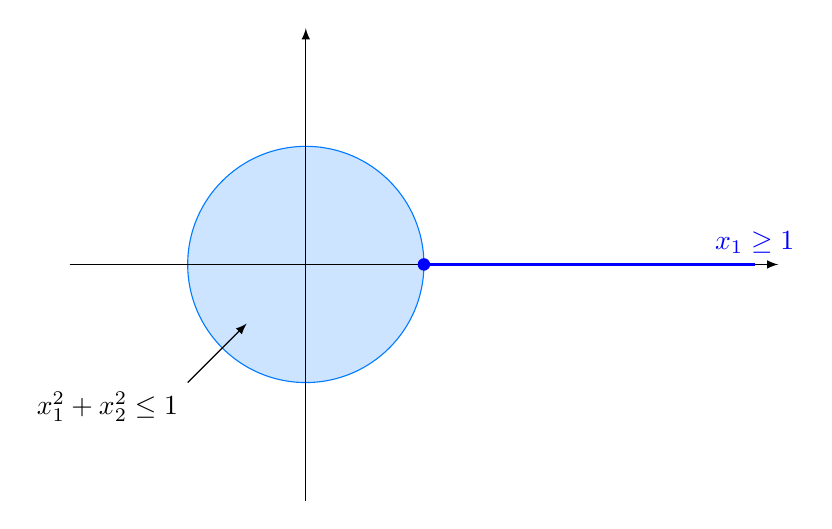
\begin{tikzpicture}[>=latex, scale=1.5]
    	\draw[color=lightblue, fill=lightblue!20] (0,0) circle (1);
    	\draw[->] (-2, 0) -- (4,0);
    	\draw[->] (0,-2) -- (0,2);
    	\draw[-latex] (-1,-1) node[below left] {$x_1^2+x_2^2\le1$} -- (-0.5,-0.5);
    	\fill[blue] (1,0) circle (1.5pt);
    	\draw[blue, line width=1.3] (1,0) -- (3.8,0) node[above] {$x_1\ge1$};
    	\end{tikzpicture}
    	
    	$(1,0)$ es solución porque es el único admisible
    	\item \db{Comprueba que la función dual viene dada por \[ \Theta(\mu)=\mu-\sqrt{1-\mu^2}. \]}
    	
    	$$\mathcal{L}(x_1,x_2,\mu_1,\mu_2)=x_2+\mu_1(1-x_1)+\mu_2(x_1^2+x_2^2-1)$$
    	Existe el mínimo de $\mathcal{L}$ y anula su gradiente. 
    	\[ \begin{array}{l}
    	\nabla_{(x_1,x_2)}=(-\mu_1+2\mu_2\mu_1+2\mu_2x_1,1+2\mu_2x_2)=(0,0)\\
    	\begin{rcases}
    	-\mu_1+2\mu_2x_1=0\\
    	1+2\mu_2x_2=0
    	\end{rcases}\begin{array}{l}
    	\longrightarrow x_1=\dfrac{\mu_1}{2\mu_2},\mu_2\neq0\\
    	\longrightarrow x_2=-\dfrac{1}{2\mu_2},\mu_2\neq0
    	\end{array}
    	\end{array} \] Si $\mu_2=0\longrightarrow\rboxed{1=0 \text{ \textcolor{red}{No}}}$
    	
    	$\begin{aligned}
    	\Theta(\mu_1,\mu_2)&=\mathcal{L}\left(\dfrac{\mu_1}{2\mu_2},-\dfrac{1}{2\mu_2},\mu_1,\mu_2\right)=-\dfrac{1}{2\mu_2}+\mu_1\left(1-\dfrac{\mu_1}{2\mu_2}\right)+\mu_2\left(\dfrac{\mu_1^2}{4\mu_2^2}+\dfrac{1}{4\mu_2^2}-1\right)\\
    	&=-\dfrac{1}{\mu_2^2}+\mu_1-\dfrac{\mu_1^2}{2\mu_2}-\mu_2+\dfrac{\mu_1^2}{4\mu_2}+\dfrac{1}{4\mu_2}=-\dfrac{1}{4\mu_2}-\dfrac{\mu_1^2}{4\mu_2}+\mu_1+\mu_2
    	\end{aligned}$
    	
    	\[ (Dual)\begin{cases}
    	\text{Maximizar} & \Theta(\mu_1,\mu_2)=-\dfrac{1}{4\mu_2}-\dfrac{\mu_1^2}{4\mu_2}+\mu_1+\mu_2\\
    	\text{Sujeto a} & \mu_1\ge0\\
    	 & \mu_2\ge0
    	\end{cases} \]
    	
    	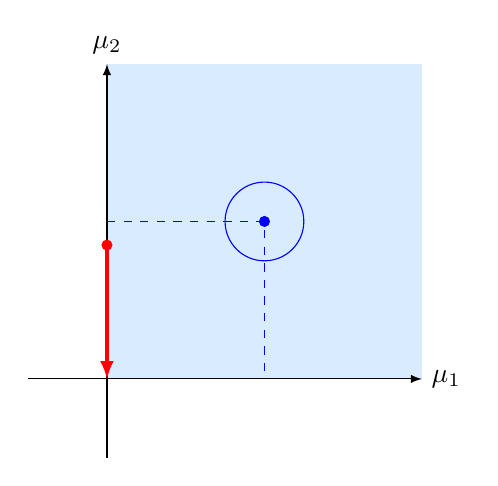
\begin{tikzpicture}[>=latex, baseline=(current bounding box.center)]
    	\fill[lightblue!15] (0,0) rectangle (4,4);
    	\draw[->] (-1,0) -- (4,0) node[right] {$\mu_1$};
    	\draw[->] (0,-1) -- (0,4) node[above] {$\mu_2$};
    	\draw[dashed, blue] (0,2) -- (2,2) -- (2,0);
    	\draw[blue] (2,2) circle (0.5);
    	\fill[blue] (2,2) circle (2pt);
    	\fill[red] (0,1.7) circle (2pt);
    	\draw[->, color=red, line width=1.2] (0,1.7) -- (0,0);
    	\end{tikzpicture}
    	
    	Miramos si hay máximo en la región $\mu_1>0,\mu_2>0$.
    	
    	\[ \nabla_{(\mu_1,\mu_2)}\Theta=\left(-\dfrac{\mu_1}{2\mu_2}+1,\dfrac{1}{4\mu_2^2}+\dfrac{\mu_1^2}{4\mu_2^2}-1\right) =(0,0)\]
    	
    	$1-\dfrac{\mu_1}{2\mu_2}\longrightarrow\mu_1=2\mu_2$
    	
    	$\begin{array}{l}
    	\Theta(\mu_1=0,\mu_2)=-\dfrac{1}{\mu_2}-\mu_2\begin{cases}
    	-\infty & \mu_2\to0\\
    	-\infty & \mu_2\to+\infty
    	\end{cases}\\
    	\lim_{\mu_1\to0}(\mu_1,\mu_2)=
    	\end{array}$
    	
    	
    	Chequeamos la condición de rango maximal
    	
    	$\begin{array}{l}
    	\nabla_{g_1}=(-1,0)\\
    	\nabla_{g_2}=(2x_1,2x_2)=\{(1,0)\}=(2,0)
    	\end{array}\qquad\begin{bmatrix}
    	-1 & 2\\
    	0 & 0
    	\end{bmatrix}=\left[\begin{array}{c:c}
    	\nabla_{g_1} & \nabla_{g_2}
    	\end{array}\right]\longrightarrow\rboxed{\rg=1\text{ \textcolor{red}{No}}}$
    	
    	El problema dual no tiene solución.
    	\item \db{Calcula $\sup\{\Theta(\mu):\mu\ge0\}$ y deduce de ello que el problema dual no tiene solución. Razona a qué es debido esto. \textit{Indicación: comprueba que no se cumple alguna de las hipótesis del teorema de dualidad fuerte.}}
    \end{enumerate}
    \item \lb{Consideremos al problema de complementariedad lineal asociado a los datos siguientes: \[ M=\begin{bmatrix}
    -2 & 1 \\
    1 & -2
    \end{bmatrix},\quad q=(1,1)^\intercal. \] Escribe las 4 matrices complementarias, dibuja los 4 conos complementarios, y deduce de ello que el problema \[ \begin{cases}
    \omega-Mz=q\\
    \omega,z\ge0\\
    \omega_j\cdot z_j=0,\quad 1\le j\le 2
    \end{cases} \]tiene 4 soluciones y calcúlalas.}
    
    $\omega\cdot\begin{bmatrix}1\\ 0\end{bmatrix}+\omega_2\cdot\begin{bmatrix}0\\1\end{bmatrix}+z_1\begin{bmatrix}2\\-1\end{bmatrix}+z_2\begin{bmatrix}-1\\2\end{bmatrix}=\begin{bmatrix}1\\1\end{bmatrix}$

\begin{tabular}{c|c|c|c|c}
Variables nulas & Variables complementarias & Matriz complementaria & Cono complementario & Solución\\ \hline \\
$\omega_1=\omega_2=0$ & $(z_1,z_2)$ & $\begin{bmatrix}2 & -1\\-1 & 2\end{bmatrix}$ & & $z_1=z_2=1$\\ \hline \\
$\omega_1=z_2=0$ & $(z_1,\omega_2)$ & $\begin{bmatrix}2 & 0\\ -1 & 1\end{bmatrix}$ & & $z_1=\dfrac{1}{2};\omega_2=\dfrac{3}{2}$\\ \hline \\
$z_1=z_2=0$ & $(\omega_1,\omega_2)$ & $\begin{bmatrix}1&0\\0&1\end{bmatrix}$ & & $\omega_1=\dfrac{3}{2},z_2=\dfrac{1}{2}$ \\ \hline \\
\end{tabular}

$\begin{rcases}
2z_1-z_2=1\\
-z_1+2z_2=1
\end{rcases}\longrightarrow\begin{rcases}
4z_1-2z_2=2\\
-z_1+2z_2=1
\end{rcases}\quad\begin{array}{l}
3z_1=3\longrightarrow z_1=1\\
z_2=2\cdot z_1-1=2\cdot 1-1=1
\end{array}$

$z_1\cdot\begin{bmatrix}2\\-1\end{bmatrix}+\omega_2\cdot\begin{bmatrix}0\\1\end{bmatrix}=\begin{bmatrix}1\\1\end{bmatrix}\longrightarrow\begin{rcases}2z_1=1\\-z_1+\omega_2=1\end{rcases}$

    \item \lb{Utiliza el algoritmo de Lemke para resolver el problema de complementariedad lineal asociado a los datos \[ M=\begin{bmatrix}
    1 & -1 \\
    -1 & 1
    \end{bmatrix},\quad q=(1,-1)^\intercal.\]}
    
    \item \lb{\textbf{El problema de la distancia mínima.} Sea $K$ la región poligonal que aparece en la Figura 1 y fijemos el punto $P_0=(-2,-1)$. Nos planteamos de encontrar el punto de $K$ que está más cerca de $P_0$, en la distancia Euclídea usual.}
    
    \begin{center}
    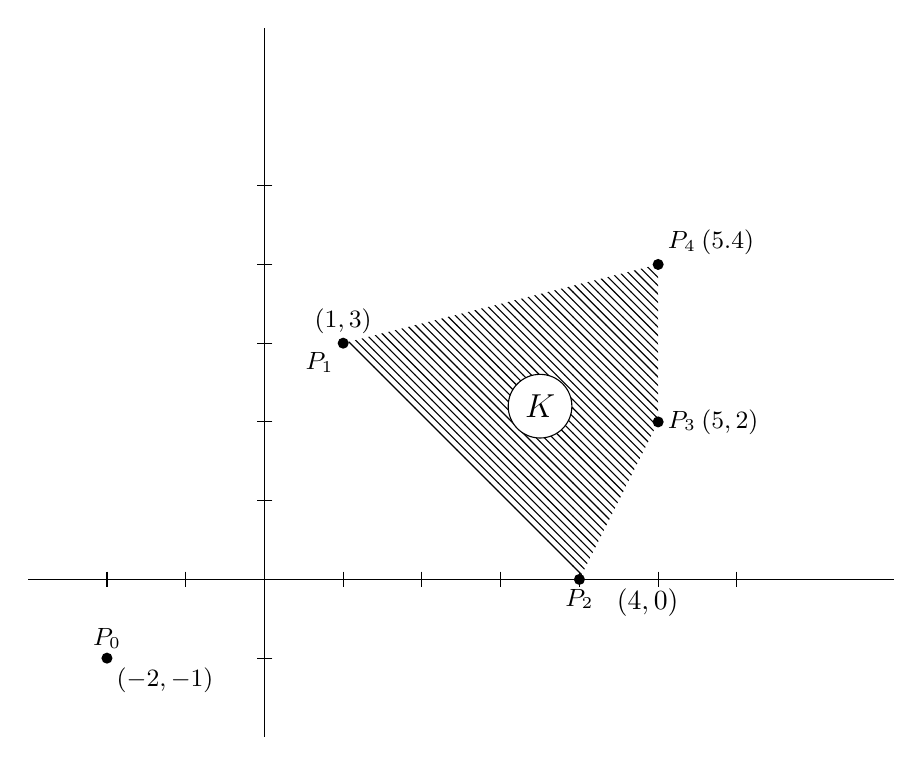
\begin{tikzpicture}
    \draw (-3,0) -- (8,0);
    \draw (0,-2) -- (0,7);
    \foreach \x in {-2,...,6}{\draw (\x,0.1) -- (\x,-0.1);}
    \foreach \y in {-1,...,5}{\draw (0.1,\y) -- (-0.1, \y);}
    % Puntos y etiquetas
        \fill (-2,-1) circle (2pt) node[above] {\small $P_0$} node[below right] {\small $(-2,-1)$};
        \fill (1,3) circle (2pt) node[below left] {\small $P_1$} node[above] {\small $(1,3)$};
        \fill (4,0) circle (2pt) node[below] {\small $P_2$} node[below right] {$\quad(4,0)$};
        \fill (5,2) circle (2pt) node[right] {\small $P_3\:(5,2)$};
        \fill (5,4) circle (2pt) node[above right] {\small $P_4\:(5.4)$};
    
        % Región sombreada (K)
        \fill[pattern=north west lines] 
            (1,3) -- (4,0) -- (5,2) -- (5,4) -- cycle;
        \node[circle, fill=white, draw=black] at (3.5,2.2) {\large $K$};
    \end{tikzpicture}
    
    \lb{Figura 1: Problema de la distancia mínima}
    \end{center}
    \lb{El problema puede formularse de la siguiente forma\footnote{El vector $(\lambda_1,\cdots,\lambda_4)$ representa un punto de $K$ y surge del Teorema de representación de un conjunto poliédrico. Para el caso sencillo en que $K$ es un triángulo, $(\lambda_1,\lambda_2,\lambda_3)$ son las coordenadas baricéntricas, que se calculan del siguiente modo: si $P_1=(x_1,y_1),\, P_2=(x_2,y_2)\, P_3=(x_3,y_3)$ son los vértices de un triángulo y $P=(x,y)$ es un punto del triángulo, entonces las coordenadas baricéntricas de $P$ son: \[ \lambda_1=\dfrac{\text{área del triángulo }PP_1P_2}{\text{área del triángulo }P_1P_2P_3},\quad\lambda_2=\dfrac{\text{área del triángulo }PP_2P_3}{\text{área del triángulo } P_1P_2P_3},\quad\lambda_3=\dfrac{\text{área del triángulo }PP_1P_3}{\text{área del triángulo }P_1P_2P_3}. \]}: \[ \begin{cases}
    \text{Minimizar} & f(\lambda_1,\cdots,\lambda_4)=(\lambda_1+4\lambda_2+5\lambda_3+5\lambda_4-(-2))^2+(\lambda_1+2\lambda_3+4\lambda_4-(-1)^2)\\
    \text{Sujeto a} & \lambda_1+\lambda_2+\lambda_3+\lambda_4=1\\
     & \lambda_j\ge0,\quad 1\le j\le 4
    \end{cases} \]Se pide:}
    \begin{enumerate}[label=\color{red}\alph*)]
    	\item \db{Utiliza la sustitución $\lambda_4=1-\lambda_1-\lambda_2-\lambda_3$ para comprobar que el problema anterior se puede reescribir como el problema cuadrático siguiente:  \begin{equation}
    	(\mathrm{PQ})\begin{cases}
    	\text{Minimizar} & (-66,-54,-20)\lambda+\dfrac{1}{2}\lambda^\intercal\begin{bmatrix}
    	34 & 16 & 4 \\
    	16 & 34 & 16 \\
    	4 & 16 & 8
    	\end{bmatrix}\lambda\\
    	\text{Sujeto a} & -\lambda_1-\lambda_2-\lambda_3\ge1\\
    	 &\lambda_j\ge0,\quad 1\le j\le 3
    	\end{cases}
    	\end{equation} donde $\mathrm{\lambda}=(\lambda_1,\lambda_2,\lambda_3)^\intercal$.}
    	
    	\item \db{Comprueba que el problema (1) es equivalente al problema de complementariedad lineal \begin{equation}
    	(\mathrm{PCL})\begin{cases}
    	\omega-Mz=q\\
    	\omega,z\ge0\\
    	\omega_j\cdot z_j=0,\quad 1\le j\le4
    	\end{cases}
    	\end{equation}donde, siguiendo la notación de clase, \[ \omega=(y,v_1,v_2,v_3)^\intercal,\quad z=(y,\lambda_1,\lambda_2,\lambda_3)^\intercal,\quad q=(1,-66,-54,-20)^\intercal \]y\[ M=\begin{bmatrix}
    	0 & -1 & -1 & -1 \\
    	1 & 34 & 16 & 4 \\
    	1 & 16 & 34 & 16 \\
    	1 & 4 & 16 & 8
    	\end{bmatrix}. \]}
    	
    	\item \db{Resuelve el problema (2) en Python mediante el algoritmo de Lemke y usando el módulo \texttt{lemkelep}.}
    	
    \end{enumerate}
    \item \lb{Consideremos el problema de optimización cuadrática siguiente: \[ (\mathrm{PQ})\begin{cases}
    \text{Minimizar} & f(x_{1},x_{2})=\dfrac{1}{2}(x_{1}^{2}+x_{2}^{2})+x_{1}+x_{2}\\
    \text{Sujeto a} & x_1+x_2\ge1\\
     & x_1,x_2\ge0
    \end{cases} \]Se pide:}
    \begin{enumerate}[label=\color{red}\alph*)]
    	\item \db{Comprueba que el problema de complementariedad lineal asociado es el correspondiente al sistema: \[ (\mathrm{PCL})\quad\begin{bmatrix}
    	y\\
    	v_{1}\\
    	v_{2}
    	\end{bmatrix}-\begin{bmatrix}
    	0 & 1 & 1 \\
    	-1 & 1 & 0 \\
    	-1 & 0 & 1
    	\end{bmatrix}\cdot\begin{bmatrix}
    	u\\
    	x_1\\
    	x_2
    	\end{bmatrix} =\begin{bmatrix}
    	-1 \\
    	1 \\
    	1
    	\end{bmatrix}\]}
    	
    	\item \db{Resuelve por el método de Lemke en Python, y usando el módulo \texttt{lemkelep}, el problema (PCL) anterior.}
    \end{enumerate}
    \item \lb{Consideremos el problema de optimización cuadrática siguiente: \[ (\mathrm{PQ})\begin{cases}
    \text{Minimizar} & f(x_1,x_2)=23x_1^2+5x_1x_2+4x_2^2+3x_1+5x_2+8\\
    \text{Sujeto a} & x_1-x_2-3\ge0\\
    & -4x_1-5x_2\le13\\
    &8x_1+14x_2\ge-9\\
    &x_1,x_2\ge0
    \end{cases} \]Se pide:}
    \begin{enumerate}[label=\color{red}\alph*)]
    	\item \db{Estudia la convexidad del problema.}
    	
    	\item \db{Escribe las ecuaciones de Karush-Kuhn-Tucker y el problema de complementariedad lineal asociados.}
    	
    	\item \db{Resuelve el método de Lemke en Python, y usando el módulo de \texttt{lemkelep}, el problema de complementariedad lineal.}
    \end{enumerate}
\end{enumerate}
\end{document}
